\documentclass[11pt]{article}

% Change "review" to "final" to generate the final (sometimes called camera-ready) version.
% Change to "preprint" to generate a non-anonymous version with page numbers.
\usepackage[review]{acl}

% Standard package includes
\usepackage{times}
\usepackage{latexsym}

% For proper rendering and hyphenation of words containing Latin characters (including in bib files)
\usepackage[T1]{fontenc}
% For Vietnamese characters
% \usepackage[T5]{fontenc}
% See https://www.latex-project.org/help/documentation/encguide.pdf for other character sets

% This assumes your files are encoded as UTF8
\usepackage[utf8]{inputenc}

% This is not strictly necessary, and may be commented out,
% but it will improve the layout of the manuscript,
% and will typically save some space.
\usepackage{microtype}

% This is also not strictly necessary, and may be commented out.
% However, it will improve the aesthetics of text in
% the typewriter font.
\usepackage{inconsolata}

%Including images in your LaTeX document requires adding
%additional package(s)
\usepackage{graphicx}

% custom packages: %
\usepackage{xcolor}
%%%%%%%%%%%%%%%%%%%%

% If the title and author information does not fit in the area allocated, uncomment the following
%
%\setlength\titlebox{<dim>}
%
% and set <dim> to something 5cm or larger.

\title{HealthQueryAgent: a task oriented dialogue system for Automated Clinical Informatics}


% Author information can be set in various styles:
% For several authors from the same institution:
% \author{Author 1 \and ... \and Author n \\
%         Address line \\ ... \\ Address line}
% if the names do not fit well on one line use
%         Author 1 \\ {\bf Author 2} \\ ... \\ {\bf Author n} \\
% For authors from different institutions:
% \author{Author 1 \\ Address line \\  ... \\ Address line
%         \And  ... \And
%         Author n \\ Address line \\ ... \\ Address line}
% To start a separate ``row'' of authors use \AND, as in
% \author{Author 1 \\ Address line \\  ... \\ Address line
%         \AND
%         Author 2 \\ Address line \\ ... \\ Address line \And
%         Author 3 \\ Address line \\ ... \\ Address line}

\author{First Author \\
  Test Edit From Overleaf Syncs \\
  Affiliation / Address line 2 \\
  Affiliation / Address line 3 \\
  \texttt{email@domain} \\\And
  Second Author \\
  Affiliation / Address line 1 \\
  Affiliation / Address line 2 \\
  Affiliation / Address line 3 \\
  \texttt{email@domain} \\}

%\author{
%  \textbf{First Author\textsuperscript{1}},
%  \textbf{Second Author\textsuperscript{1,2}},
%  \textbf{Third T. Author\textsuperscript{1}},
%  \textbf{Fourth Author\textsuperscript{1}},
%\\
%  \textbf{Fifth Author\textsuperscript{1,2}},
%  \textbf{Sixth Author\textsuperscript{1}},
%  \textbf{Seventh Author\textsuperscript{1}},
%  \textbf{Eighth Author \textsuperscript{1,2,3,4}},
%\\
%  \textbf{Ninth Author\textsuperscript{1}},
%  \textbf{Tenth Author\textsuperscript{1}},
%  \textbf{Eleventh E. Author\textsuperscript{1,2,3,4,5}},
%  \textbf{Twelfth Author\textsuperscript{1}},
%\\
%  \textbf{Thirteenth Author\textsuperscript{3}},
%  \textbf{Fourteenth F. Author\textsuperscript{2,4}},
%  \textbf{Fifteenth Author\textsuperscript{1}},
%  \textbf{Sixteenth Author\textsuperscript{1}},
%\\
%  \textbf{Seventeenth S. Author\textsuperscript{4,5}},
%  \textbf{Eighteenth Author\textsuperscript{3,4}},
%  \textbf{Nineteenth N. Author\textsuperscript{2,5}},
%  \textbf{Twentieth Author\textsuperscript{1}}
%\\
%\\
%  \textsuperscript{1}Affiliation 1,
%  \textsuperscript{2}Affiliation 2,
%  \textsuperscript{3}Affiliation 3,
%  \textsuperscript{4}Affiliation 4,
%  \textsuperscript{5}Affiliation 5
%\\
%  \small{
%    \textbf{Correspondence:} \href{mailto:email@domain}{email@domain}
%  }
%}

\begin{document}
\maketitle
\begin{abstract}
% What does this paper add
In this paper we describe \textbf{HealthQueryAgent,} a Task-Oriented Dialogue (TOD) for performing population health management operations. We deploy the system in a familiar chat interface embedded within an existing population health management platform and run experiments to determine it's utility to a diverse userbase of 2,000 analysts and clinicians querying data from over 1.4M patients. We evaluate the agent's capacity to autonomously handle a range of health informatics tasks. We compare a range of frontier LLMs on a benchmark comprised of real-world user (question, query) pairs, and find (TBD). % todo

% Analysing healthcare data can be an arduous and error-prone task when done manually. 
The aim of population health analysis is for a user to generate some knowledge from a database by conducting a database query to access information regarding a set of specified patients. 
% Three examples are: listing patients who meet some criteria; calculating the rate of a condition within a subpopulation; and measuring the performance of their organisation according to some metrics.
Specialist analysts are needed to translate clinical queries into database ones, imposing a steep cost and introducing a considerable delay. We hypothesise a system for automatically performing this translation in an interpretable fashion could drastically reduce both the cost and the latency to performing population health analysis, and enable clinicians to rapidly generate actionable knowledge from clinical data.

% This document is a supplement to the general instructions for *ACL authors. It contains instructions for using the \LaTeX{} style files for ACL conferences.
% The document itself conforms to its own specifications, and is therefore an example of what your manuscript should look like.
% These instructions should be used both for papers submitted for review and for final versions of accepted papers.
\end{abstract}


\begin{figure}[t]
  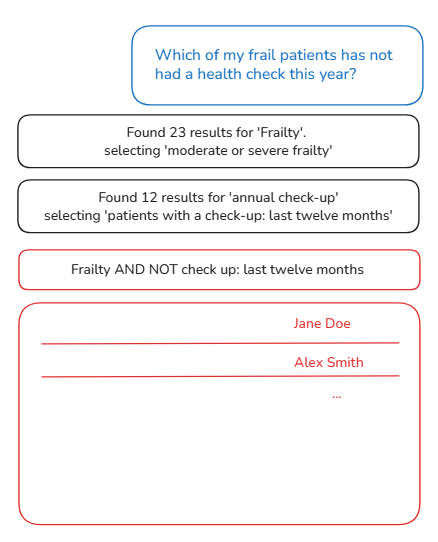
\includegraphics[width=\columnwidth]{content/chat_diagram.PNG}
  \caption{A figure with a caption that runs for more than one line.
    Example image is usually available through the \texttt{mwe} package
    without even mentioning it in the preamble.}
  \label{fig:experiments}
\end{figure}


\section{Introduction}

% focus has been elsewhere
Healthcare organisations collect vast quantities of healthcare data, however at present it would be difficult to argue that this data is used to it's \textit{full potential}. Whilst there has been a concerted effort from machine learning researchers to automate various extractive medical tasks such as clinical coding and radiology report generation, relatively few studies have investigated how to maximise clinical use of this information: leaving large population health benefits `on the table' so to speak.

% Ensure this is rendered on page 2.
\begin{figure*}[t]
  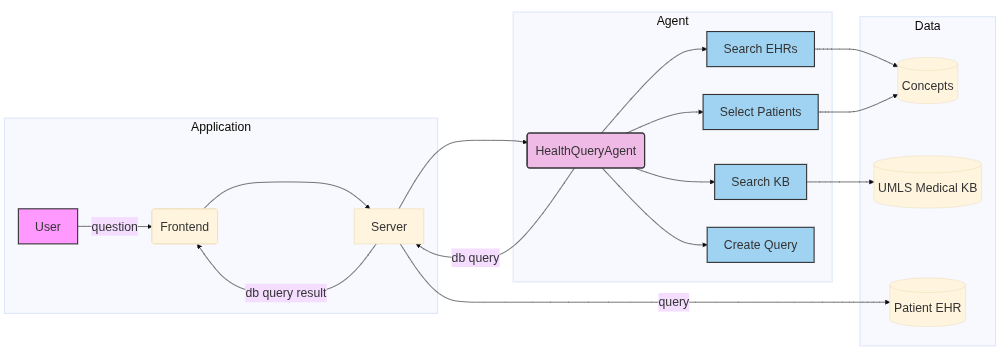
\includegraphics[width=\linewidth]{content/system_diagram3.png}
	\caption{System diagram showing a subset of HealthQueryAgent's tools. The agent must enact multi-step plans using a concept database and a medical knowledge base to create an analysis query, which is then passed to the user who will be able to view the retrieved results. To ensure privacy, the agent's tools cannot access the Patient EHR database. The user may interactively refine the query by conversing with the agent, for instance prompting it to modify it's results or asking follow up questions.}
	\label{fig:system-diagram}
\end{figure*}

% Formulation
\subsection{Task}
This paper attempts to generate population health queries from real-world user questions.
This is a complex challenge as it encompasses a wide range of abilities: determining the user's intent (semantic parsing); disambiguating complex and often overloaded medical language; retrieving and selecting the appropriate medical concepts; and finally creating a query which best operationalises the user's goal.
We ask the following three research questions:

\textbf{RQ1:} Is it possible to automate the mapping from a clinical question to a database query? Formally, given a clinical user's question $Q$ and a database of patients, medical concepts (codes) and code occurrences (events) $DB$,

  $$ DB = (patients, concepts, events) $$

can we construct a system, $M$, which maps unseen user questions to an appropriate answer $A$?

  $$ M(DB): \mathcal{Q} \rightarrow \mathcal{A} $$

\textbf{RQ2:} Can we maintain the agent's performance over long, multi-stage tasks, and between tasks?

\textbf{RQ3:} Does providing an external knowledge base (KB) enhance the agent's ability to generate queries? Prior studies show that LLMs perform worse on rarer medical concepts. Does an external KB benefit queries for rare medical concepts more than common ones?

\subsection{Task-Oriented Dialogue and LLM Agents}
% todo: make more relevant to our work.
Task-Oriented Dialogue (TOD) systems are those in which an agent converses with a user to perform a task, such as booking a flight. This is in contrast to open-domain dialogue, which is not limited to the domain of any specific task. A sub-task of TOD is semantic parsing, the process of creating logical interpretations of an instruction / utterance in the context of the dialogue thus far in order to determine what action to perform next.

Traditional TOD systems typically consist of a pipeline of distinct modules, each with a specific responsibility. A typical modular architecture might include a component for understanding the user's intent and extracting structured information from it (NLU); a component for tracking the state of the dialogue (DST); a policy module for determining the next action; and a final natural languge generation model for synthesising a response.  

As pointed out in \citet{yi_a_survery_2024}, the propogation of errors between modules hampers the performance of these systems, and they have largely fallen to the wayside in favour of systems which utilize a single sequence-to-sequence model to perform the entire task. Examples of the latter include \citet{wen_network-based_2017}, who developed a novel NN architecture; Andreas et al., who were the first to treat TOD as a data flow graph in which the agent iteratively generates the program as the conversation progresses \citet{andreas_task-oriented_2020}. \citet{hoesseini-asl_2020} et al. created SimpleTOD, an end-to-end architecture utilising only one LM, GPT-2, to perform all aspects of task completion including database calls, with the results concatenated to the context.
In sum, recent progress in TOD systems has been to move away from modular architectures and towards unified ones, epitomised by the SimpleTOD approach, which uses only a finetuned LLM. 


% Two key challenges in TOD maintaining coherence over long multi-turn conversations (\citet{laban_llms_2025}), as well as identifying when f under-specified questions\cite{gan_clarq-llm_2024}
In 2025, the most commonl form of TOD agents, referred to simply as `agents', are coding ones such as Claude Code, which can autonomously perform relatively long-horizon programming tasks issued via a command-line interface\cite{METR}.
%LLM agents (agents) refer to instruction-tuned models which are augmented with tools (functions) which enable them to take actions within an environment e.g. retrieving information from Wikipedia in order to obtain an answer \cite{yao_reac_2023}.
Similar to SimpleTOD executing database commands based on autoregressive modelling of the user's belief state, agents issue what's known as `tools-calls' through autoregressive language modelling. This is referred to as the `ReACT' paradigm, after the seminal paper from \citet{yao_reac_2023}.

Agents can determine their course of action dynamically as opposed to performing tasks in a predefined sequence or pipeline.
% In a task-oriented setting, they implicitly perform the NLU, DST, policy, and generation aspects which previously would have been distinct modules.
% This change allows agents to dynamically interact with the environment and to change course as they progress and receive new information, enabling them to excel at complex tasks like programming where purely generative models typically fail.
% sole task is to retreive information, a paradigm described as `agentic information retrieval' by \citet{zhang_agentic_2025}.


\subsection{Health Informatics}
% Informatics
Health informatics is an interdisciplinary field at the intersection of data analytics and medicine, and entails improving the health outcomes through the broad use of clinical data. Informatics tasks include: writing database queries to select cohorts of patients meeting certain criteria, measuring the performance of interventions, and developing tools for clinicians to better access data. 

% EHR
The data used in healthcare informatics is stored in electronic healthcare records (EHR). Personal EHR are a rich store of information, often containing thousands of recorded medical codes dating back to a persons's birth. These records are used to great effect in large health organisations such as the NHS, where this data enables clinicians to proactively identify people's needs and to provide targeted interventions, through the use of digital clinical decision support systems (CDSS).


% Recent developments in data 
The quality of the recorded data has improved dramatically due to various incentive structures put in place, such as the mandate that providers and hospitals in the United States must exhibit `meaningful use' of the EHR in order to be eligible for Medicare and Medicaid funding, which has been fully in effect since 2016\footnote{https://www.healthit.gov/faq/what-meaningful-use}. In the UK similar incentives for good medical coding exist, with additional funds allocated to reimburse organisations which handle more complex cases, conditional on the diagnoses and procedures being properly coded.

% todo graphic of the EHR?

% Epidemiology
The ability of public health institutions to identify and respond to emergencies depends on their ability to aggregate and interpret information about the situation on the ground. Whilst digital records simplify the aggregation of said information, creating the correct database queries to analyse the data often requires the assistance of programmers, as CDSS tools typically provide limited analysis capabilities.


% TODO diagram of cohort selection (it's just a 2D space!) -- ref. the 3B1B video on Bayes' theorem.

We describe \textbf{HealthQueryAgent}, an agentic, task-oriented-dialogue (TOD) system for generating interpretable medical database queries using generative language models. We demonstrate the utility of this system through a beta deployment in NHS Nottingham and Nottinghamshire, where the system is used by members of both the clinical and analyst staff.
In our beta deployment, we present HealthQueryAgent via a chat interface embedded into an existing web platform for population health management, enabling the clinician to collaborate with the agent to refine the analysis. % todo: hard to parse the last sentence.

% Interpretability
For the results of an automated querying system to be actionable, they must first be interpretable. Specifically, generated database queries must be understandable to the user; whilst SQL is ubiquitous amongst analysts, clinicians will struggle to verify that an SQL query is correctly expressing their intent. To work around this limitation, we limit cohort selection queries (the predominant type of query) to a subset which can be expressed using a composition of only three logical operations: \texttt{AND, OR, AND NOT}. For clinician facing CDSS the tradeoff of expressivity for interpretability could be worthwile compared to text-to-SQL based systems, whose queries cannot be easily verified by non-programmers.

% is that our system generates queries in an interpretable intermediate representation (IR). In order to make decisions based on the results of the generated query, it is critical that the query itself can be checked logically by the user.In the case of an analyst generating SQL is appropriate, however non-programmers will have difficulty validating the correctness of SQL queries. 

 %clinicians can understand the underlying logic; something which is arguably not possible with text-to-sql pipelines used in other systems in the literature. We address this by expressing queries using a simple intermediate representation (IR) consisting of three first-order logic operations: \texttt{AND,OR,NOT} as well as the concept of a fraction. This IR is programmatically mapped to an SQL query and provides a simple mechanism for non-programmers to ensure that the query is logically correct- a key requirement for actionable analyses.

% Local context
In the context of the UK, where this study takes place, our National Health Service has announced three major shifts in it's operations\footnote{https://www.england.nhs.uk/digitaltechnology/the-single-patient-record/}:

\begin{enumerate}
	\item hospital to community
	\item sickness to prevention
	\item analogue to digital
\end{enumerate}

HealthQueryAgent fits squarely within these aims. By enabling primary (community) care physicians to proactively pin-point people who need assistance, the burden can be shifted away from expensive secondary care services (hospitals / inpatient facilities).


% SEMANTIC PARSING
Semantic Parsing is the task of parsing a user's utterance into a logical statement.

% TEXT TO SQL (ziletti 2024,2025)
\citet{ziletti_retrieval_2024} \citet{ziletti_generating_2025}

\section{Related Work}

Our proposed agent-based, task-oriented dialogue system for medical database querying sits at the intersection of three strands of research: Task-Oriented Dialogue, agent-based information retrieval, and text-to-SQL.

\subsection{Text-to-SQL}
Text-to-SQL is the task of operationalising a question by mapping it to a Structured Query Language (SQL) script.

Medical applications of text-to-SQL have largely focussed on translating natural language queries into database ones directly as part of health analyst workflows \citet{ziletti_retrieval_2024}.

\section{Method}
% A method is like a recipe.
In this section we describe the HealthQueryAgent system and development process.

% \subsection{Automated testing} ...

\subsection{Workflows}
...

\subsection{Tools}
The agent has a fixed set of tools provided in the industry standard json tools format.
The tools contain brief descriptions of their function, and are mapped 1:1 with Python functions internally, using a switch-case statement.

\subsubsection{Return}
The agent may return a result in the form of a URL link showing the user the result of the generated query, as well as the query itself.
The output modes include

\begin{table}[t]
\centering
\begin{tabular}{|p{2cm}|p{5cm}|}
\hline
	Output mode & Sample requests \\
\hline
\hline
	Patient List	& show me the \textcolor{blue}{dementia status} for people with moderate or severe frailty; \\
			& Hip fracture; \\ 
\hline
	Cohort Statistics 	& How many patients are on \textcolor{red}{PERT}? \\
				& What's the rate of ADHD in people with Autism? \\
				& Show me the distribution of \textcolor{teal}{ages} for \textcolor{orange}{dementia patients.} \\
\hline
	KPIs 	& How's \textcolor{brown}{Saxon Cross} doing on admissions avoidance? \\
		& Is Nottingham West doing better than East on diabetes management? \\	
\hline
\end{tabular}
\caption{
	Queries with named entities highlighted in various colours.
	There a number of matching entities types and the agent must infer from the query both the appropriate entity and the appropriate entitiy type.
	For instance for the phrase `\textcolor{blue}{dementia status}' is a request for a report (a specific columnar view of the patient list) but there also exist related
	concepts (e.g. \textcolor{orange}{Dementia}) and KPIS which the model must determine are irrelevant to the query despite their lexical similarity.
	\\ \textbf{Takeaway:} selecting entities to use the in the answer requires sophisticated interpretation of the user intent.  
}
\label{tab:sample-queries}
\end{table}



\subsubsection{Search}
To enable the agent to access the relevant contents of various tables, we provide it with a search tool.
The tool takes two arguments: a key, which is used for a simple substring match, and a mode, which is used to determine the type of entity being searched
for.

\begin{table}[t]
\centering
	\begin{tabular}{|p{2cm}|p{5cm}|}
\hline
	Entity Type & Sample entities \\

\hline
\hline
	Concepts 	& \textcolor{orange}{Dementia} \\
	 	        & \textcolor{red}{Pancreatic Enzyme Replacement Therapy} \\
			& Diabetes - L12M \\
			& 2+ hospital admissions L12M \\
			& Hip fracture \\ 
\hline
	Locations	& \textcolor{brown}{Saxon Cross General Practice;}\\	
			& Nottingham West; \\
			& Orchard Surgery; \\
\hline
	KPIs		& \% of diabetics whose HBa1c is 48mmol/mol or lower; \\
	 		& \% of medication reviews for those on the end of life register; \\	
\hline
	Reports		& \textcolor{blue}{Dementia:} \\
			& Age | Sex | MoCA score | \\
			& Frailty: \\
			& Age | Sex | Barthel independence score | clinical frailty score | history of falls \\
\hline
	Statistics	& \textcolor{teal}{Age bands} \\
			& Diagnoses \\
			& Admissions \\
\hline
\end{tabular}

\caption{
	A sample of entities which HealthQueryAgent needs to marshal in order to generate it's answer queries.
	`L12m' refers to data recorded in the the last 12 months.
	`HBa1c' is a blood sugar test used to measure the performance of diabetes treatments, the specific value corresponds to the clinical threshold for `well-controlled'.
%	\textbf{Takeaway}: the agent must retrieve local data to complete it's task.
}
	\label{tab:sample-entities}
\end{table}


\subsection{Privacy preserving design}
Personal health information cannot be processed by third-party APIs.
To ensure that no personal data can be accessed by the agent, we create a selection of database tools which do not provide access to the `Patient' table, or any derivates thereof; the agent is limited to generating a \textit{query} for patient information, which is executed by the user according to their resective level of permissions, as shown in Figure \ref{fig:system-diagram}.


\section{Experimental Setup}
% What experiments did you run to test your hypotheses, and why?
To test the capabilities of our agent, we use a selection of 100 real-world dialogues and judge the agent's performance in them compared to an expert analyst.

We grade each agent according to the following two measures: \textbf{parsing}: does the expert analyst agree with the agent's interpretation of the user intent? \textbf{accuracy}: did the agent select the same segment of patients as the expert analyst?

\section{Results}
% (descriptive) What did our experiments show?


\section{Conclusion}
% What did we take away from these results?


\begin{table}[t]
\centering
\begin{tabular}{|l|c|c|}
\hline
	& user & agent \\
\hline
	dialogues	& XXX & YYY \\
	utterances	& XXX & YYY \\
	words 		& XXX & YYY \\
\hline
\end{tabular}
\caption{Statistics of the HealthQueryAgent conversations.}
\label{tab:results}
\end{table}



\section*{Limitations}

\section{Ethics Statement}
Population health management is a serious task, and the use of AI warrants proper ethical consideration.

To address the ethical concerns regarding this work, let us consider the mechanisms by which such a system could cause harm.

Since the agent cannot access patient data, we deem the risk of leaking PII to be limited to the uploading of patient information into the dialogue by a user and explicitly warn users at the beginning of each chat to not upload any PII.

The core risk we identify is that the system generates an incorrect output, leading to a clinician to be misled about the status of one or more patients, resulting in harm to those patient(s) due to the clinician taking a different course of action that they otherwise might, a risk which takes the following forms:

\begin{enumerate}
	\item Errors in selecting concepts
	\begin{enumerate}
		\item due to incorrect disambiguation e.g. of an overloaded terms
		\item due to lack of specialist knowledge e.g. multiple competing database concepts for the same utterance   
		\item due to under-specification of the user intent
		\item due to confabulation
		\item due to random chance
	\end{enumerate}
	\item Errors in formulating queries
	\begin{enumerate}
		\item due to semantic parsing errors 
		\item due to random chance
	\end{enumerate}
\end{enumerate}

\textbf{Errors in selecting concepts:}
Recall that clinical concepts refer to one or more medical codes, possibly with accompanying logic, such as a time-window: `COVID in the last six months' is a concept, for instance.

Errors in selecting concepts due to the presence of multiple retrieved concepts for a given search are a common error-mode of our system. Many of these concept selection sub-tasks require knowledge of the specific context in which a clinician or analyst created the concept in the first place, making it challenging for the LLM to select the correct one.

Additionally, LLMs have been known to confabulate/hallucinate when confronted with information they don't understand, something we have observed when handling highly-local knowledge internal to the NHS.

\textbf{Errors in formulating queries:}
Formulating the correct AND/OR query for a given utterance is of central importance, as it dictates the cohort of patients which will be selected.
Conditional on the correct concepts being selected and the user's intent being clear, we find that the tested LLMs consistently generate the correct logical queries.
In cases where the user intent is unclear, semantic parsing issues become more frequent. Due to the nature of LLMs, we cannot rule out these errors entirely; indeed, the fact that the LLM generates queries highly consistently may lull the user into a false sense of security, leading them to unthinkingly accept a result and thereby generating false knowledge. Our training material for users will note this fact and urge them to remain suspicious of the generated output.

\textbf{Ethics Summary:} we identify incorrect answers might lead to real-world harm. We address this concern by making the entire answer generation process transparent and interpretable, including the database queries which are generated in a simple, interpretable representation, enabling non-programmers to audit them.


\section*{Acknowledgments}
We thank the NHS Nottingham Data Management Team for their expertise and contributions to this project. We thank Anthony Dranfield and Ben Clarke for their assistance with the eHealthScope platform and database, and Carl Davis for organising the collaboration.

\bibliography{references}

\appendix

% \section{Example Appendix}
% \label{sec:appendix}
% This is an appendix.

\end{document}
